\documentclass{standalone}
\usepackage{tikz}
\usetikzlibrary{arrows.meta}

\begin{document}

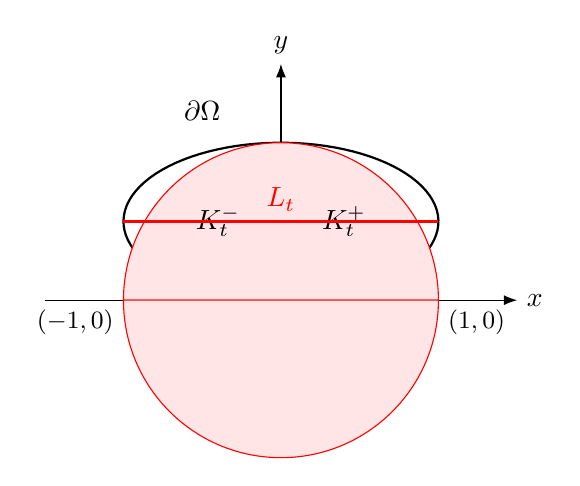
\begin{tikzpicture}[scale=2]

% Axes
\draw[-Latex] (-1.5,0) -- (1.5,0) node[right] {$x$};
\draw[-Latex] (0,-0.5) -- (0,1.5) node[above] {$y$};

% Points on the x-axis
\node at (-1,0) [below left] {\small $(-1,0)$};
\node at (0,0) [below] {\small $(0,0)$};
\node at (1,0) [below right] {\small $(1,0)$};

% Outer curve \partial\Omega
\draw[thick] plot[domain=-90:270,samples=100] ({cos(\x)}, {sin(\x)/2 + 0.5});
\node at (-0.5,1.2) {\(\partial\Omega\)};

% Inner semicircles C_r^- and C_r^+
\draw[thick] (-0.8,0) arc (180:0:0.8);
\draw[dashed] (0.8,0) arc (0:-180:0.8);
\node at (-0.6,-0.3) {\(C_r^-\)};
\node at (0.6,-0.3) {\(C_r^+\)};

% Semicircular regions K_t^- and K_t^+
\filldraw[draw=red, fill=red!10] (-1,0) arc (180:0:1) -- cycle;
\node at (-0.4,0.5) {\(K_t^-\)};
\filldraw[draw=red, fill=red!10] (1,0) arc (0:-180:1) -- cycle;
\node at (0.4,0.5) {\(K_t^+\)};

% Horizontal line segment L_t
\draw[red, thick] (-1,0.5) -- (1,0.5) node[midway, above] {\(L_t\)};

\end{tikzpicture}

\end{document}